\documentclass[a4paper,10pt,onecolumn]{article}
\usepackage{cv}

\begin{document}

\begin{minipage}[c]{0.7\textwidth}
    {\fontsize{30}{36}\selectfont \textbf{\color{primary} Maciej \color{accent} Flaga}} \\[10pt]
    \faEnvelope \ \href{mflaga@student.agh.edu.pl}{mflaga@student.agh.edu.pl} \\
    \faPhone \ +48 576 396 580 \\
    \faMapMarker* \ Rząska, Poland
\end{minipage}
\begin{minipage}[c]{0.3\textwidth}
    \raggedleft
    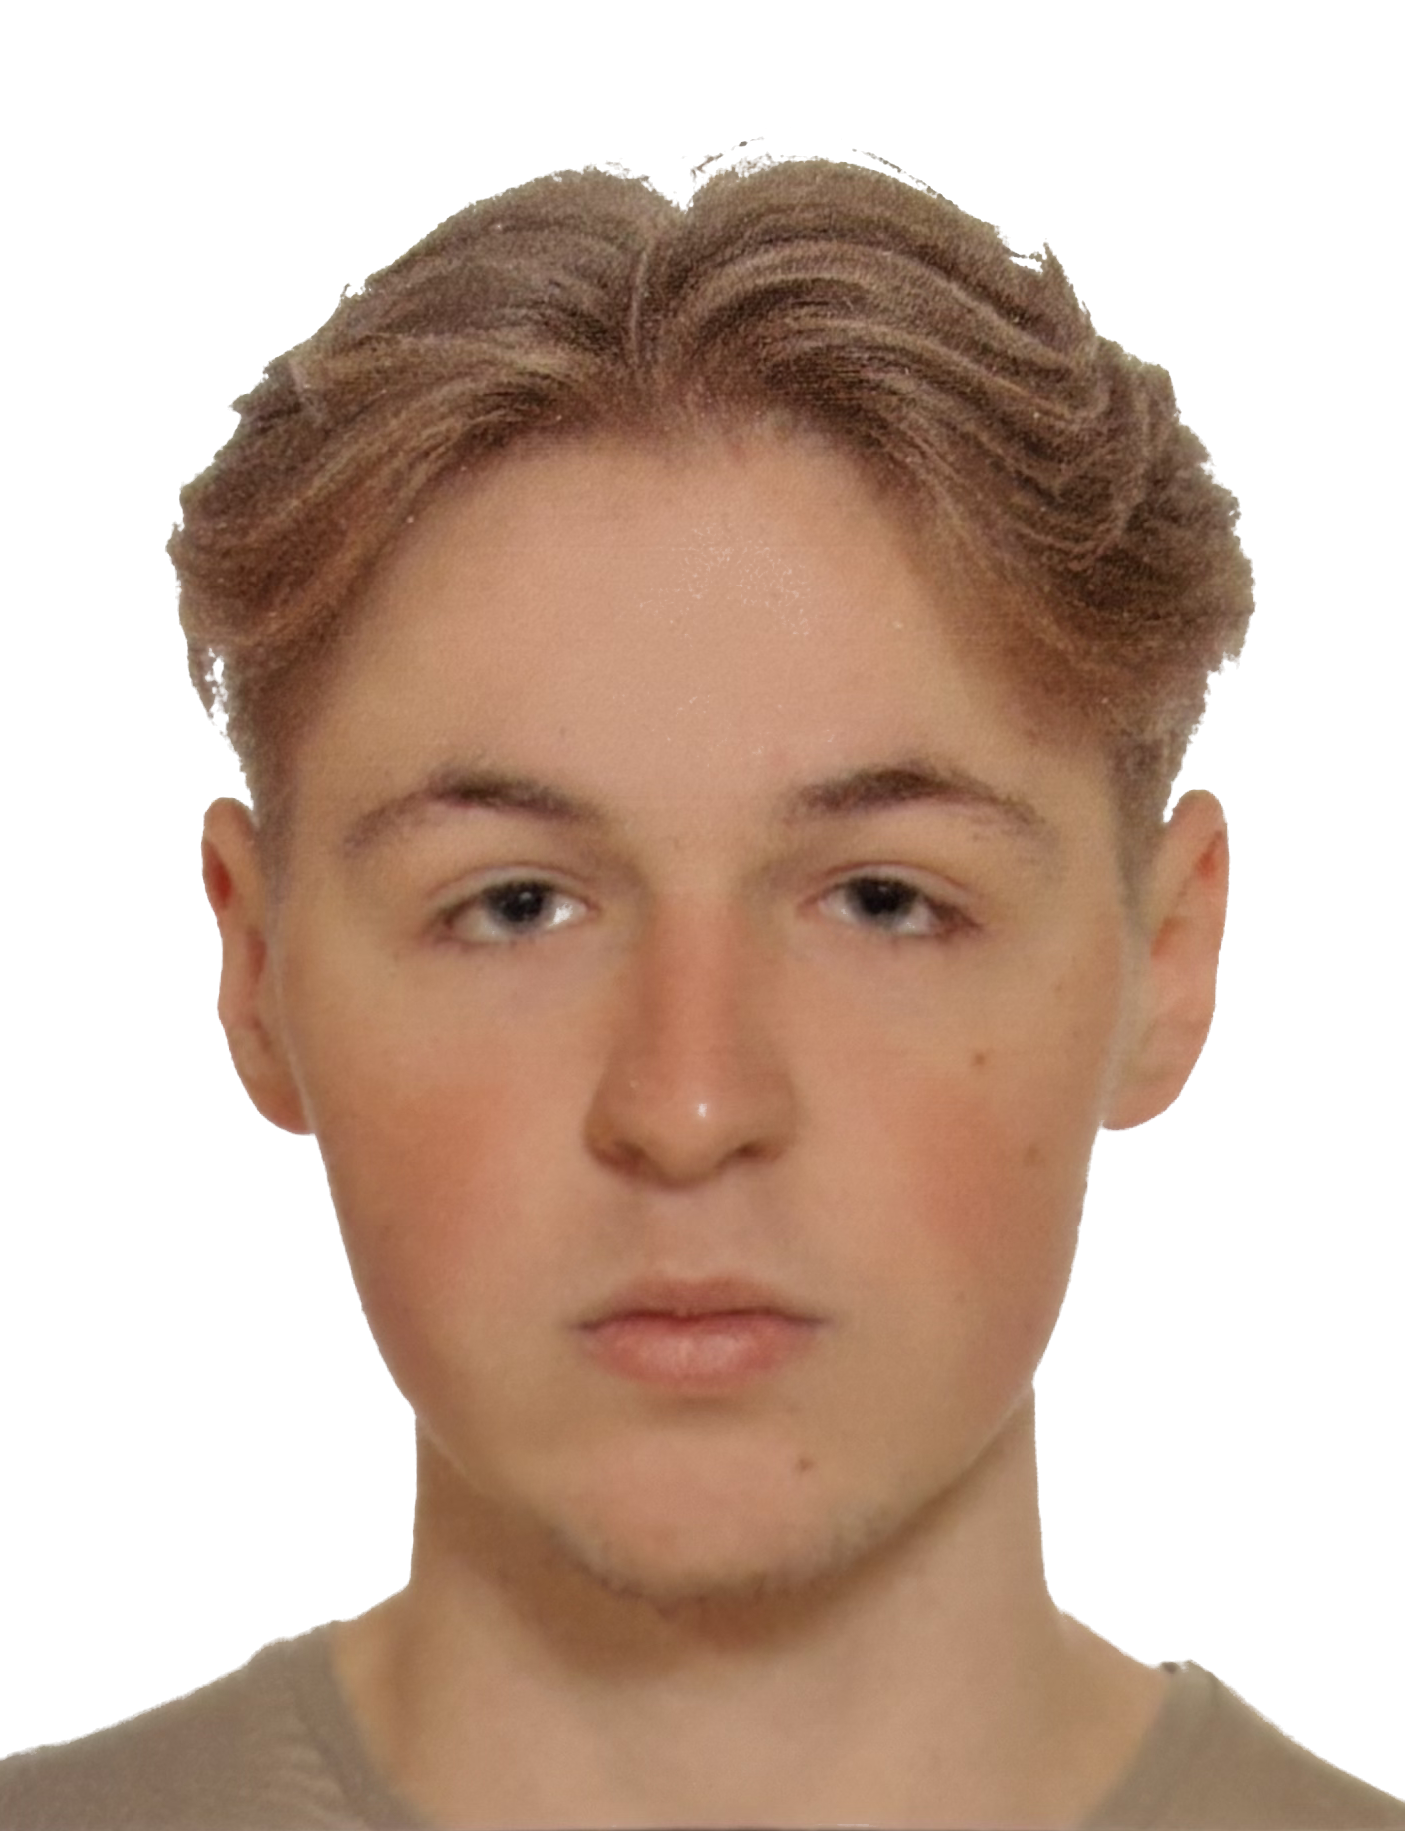
\includegraphics[width=3.5cm, height=3.5cm, keepaspectratio]{img/zdj.png} 
\end{minipage}

\section{Profile}

Undergraduate student in Nanoengineering of Materials with a strong interest in computational physics, numerical simulations, and theoretical aspects of materials science. Experienced in C/C++, Python and CUDA for scientific computing. Seeking to develop skills in simulation, modeling, and data analysis.

\vspace{10pt}

\section{Education}

\eduentry
    {img/agh.png}
    {Student}
    {AGH University of Krakow}
    {Kraków, Poland}
    {Oct. 2023 -- ongoing}
    {Faculty of Physics and Applied Computer Science\\Field: Nanoengineering of Materials\\Specialization: Modeling}

\section{Software and language skills}

\begin{minipage}[t]{0.48\textwidth}
    \textbf{\large Software}
    \begin{itemize}[leftmargin=2.5em, labelsep=0.5em]
        \imgitem{img/soft/cpp.png}{Proficient in C/C++}
        \imgitem{img/soft/py.png}{Proficient in Python (NumPy, Matplotlib, pandas)}
        \imgitem{img/soft/latex2.png}{Proficient in \LaTeX}
        \imgitem{img/soft/cuda.png}{Experienced with CUDA C++}
        \imgitem{img/soft/matlab.png}{Fairly experienced with Matlab}
        \imgitem{img/soft/linux.png}{Basic knowledge of the Linux OS}
    \end{itemize}
\end{minipage}
\hfill
\begin{minipage}[t]{0.48\textwidth}
    \textbf{\large Languages}
    \begin{itemize}[leftmargin=2.5em, labelsep=0.5em] 
        \flagitem{img/flag/pl.png}{Polish --  Native}
        \flagitem{img/flag/gb.png}{English -- Fluent}
        \flagitem{img/flag/de.png}{German -- Basic}
    \end{itemize}
    \textbf{\large Certificates}
    \begin{itemize}[leftmargin=2.5em, labelsep=0.5em]
        \imgitem {img/soft/acert.png}{ACERT Business English C1 (2025)}
    \end{itemize}
\end{minipage}

\section{Academic Projects}


\projentry
    {\href{https://github.com/mflagga/cuda-cfd-solver}{Mass Transport Simulation}}
    {Developed a GPU-accelerated Computational Fluid Dynamics (CFD) engine to simulate incompressible flow and mass transport using the \textbf{Navier-Stokes} and \textbf{Advection-Diffusion} equations. Implemented the Stream Function-Vorticity formulation using Finite Difference Methods, solving the resulting linear systems via \textbf{parallelized Red-Black Gauss-Seidel relaxation} custom \textbf{CUDA} kernels. The simulation features a \textbf{Crank-Nicolson scheme} for stable time-stepping of mass distribution and integrates a \textbf{Python/FFmpeg} pipeline to render high-framerate visualizations of velocity fields and concentration heatmaps.}

\projentry
    {\href{https://github.com/mflagga/wave-vis}{(2+1)D Wave Equation Simulation}}
    {Developed a high-performance visualizer for the (2+1)D wave equation by deriving an exact analytical solution via \textbf{separation of variables} and \textbf{Fourier series expansion}. Implemented the numerical evaluation of the double infinite series using \textbf{CUDA C++}, optimizing performance by parallelizing the summation loops on the GPU to handle high-resolution spatial grids. The project features a fully automated pipeline that orchestrates the C++ backend, \textbf{Python} \textbf{(Matplotlib)} for 3D surface plotting, and \textbf{FFmpeg} for video rendering using a custom \textbf{Makefile}.}

\newpage
\section{Job Experience}

\jobentry
    {Production line worker}
    {YK Poland Sp. z o.o.}
    {Modlniczka, Poland}
    {Jul. 2024 -- Sep. 2024 (3 months)}
    {Executed the complete production cycle of metal photo frames, including profile cutting, assembly, shrink-wrapping, and final packaging.}

\jobentry
    {Production line worker}
    {BMK Professional Electronics GmbH}
    {Augsburg, Germany}
    {Jul. 2023 -- Sep. 2023 (3 months)}
    {Performed manual PCB assembly, operated the reflow soldering process, and handled board preparation involving masking and machine-assisted dispensing.}
    
\begin{comment}
\section{Personal skills}
\begin{itemize}[itemsep=1pt, topsep=0pt, leftmargin=1.5em]
    \item Analytical thinking and problem solving
    \item Fast learning
\end{itemize}
\end{comment}

\begin{comment}
\section{Certificates}
\begin{itemize}[itemsep=1pt, topsep=0pt, leftmargin=1.5em]
    \item Acert Business English C1 (2025)
\end{itemize}
\end{comment}

\section{Interests}

\begin{minipage}[t]{0.48\textwidth}
    \textbf{\large Scientific}
    \begin{itemize}[itemsep=1pt, leftmargin=1.5em]
        \item Scientific computing
    \end{itemize}
\end{minipage}
\hfill
\begin{minipage}[t]{0.48\textwidth}
    \textbf{\large Non-scientific}
    \begin{itemize}[itemsep=1pt, leftmargin=1.5em]
        \item Climbing
    \end{itemize}
\end{minipage}

\end{document}
